\documentclass{article}%
\usepackage[T1]{fontenc}%
\usepackage[utf8]{inputenc}%
\usepackage{lmodern}%
\usepackage{textcomp}%
\usepackage{lastpage}%
\usepackage{xcolor}%
\usepackage{tikz}%
\usepackage[left=0.5in, right=0.5in, top=1in, bottom=1in]{geometry}%
%
\definecolor{P0}{HTML}{daf79c}%
\definecolor{P1}{HTML}{9cf7e0}%
\definecolor{P2}{HTML}{9ce0f7}%
\definecolor{P3}{HTML}{f5eaae}%
%
\begin{document}%
\normalsize%
\section{SJN Scheduling}%
\label{sec:SJNScheduling}%

        \section*{Introduction}
        The "Shortest-Job-Next" (SJN) algorithm is one of the scheduling algorithms in operating systems designed to manage processes in a multitasking system. In this algorithm, processes that have a shorter execution time are executed earlier than other processes. In other words, SJN tries to prioritize the shortest process to minimize the waiting time of the whole system.
        %
\subsection{Time 0: Process P0}%
\label{subsec:Time0ProcessP0}%


\begin{figure}[h!]%
\centering%
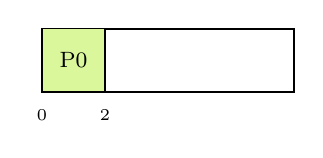
\begin{tikzpicture}%
\draw[thick] (0,0) rectangle (3.200000, 0.800000);%
\node[draw, minimum width=0.800000cm, minimum height=0.800000cm, text centered, fill=P0, font=\fontsize{8}{9}\selectfont] at (0.400000, 0.400000) {P0};%
\node[font=\fontsize{6}{8}\selectfont] at (0.000000, -0.3) {0};%
\node[font=\fontsize{6}{8}\selectfont] at (0.800000, -0.3) {2};%
\end{tikzpicture}%
\end{figure}

%
\subsection{Time 2: Process P2}%
\label{subsec:Time2ProcessP2}%


\begin{figure}[h!]%
\centering%
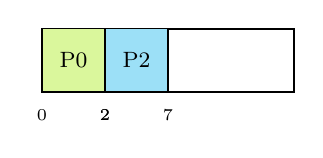
\begin{tikzpicture}%
\draw[thick] (0,0) rectangle (3.200000, 0.800000);%
\node[draw, minimum width=0.800000cm, minimum height=0.800000cm, text centered, fill=P0, font=\fontsize{8}{9}\selectfont] at (0.400000, 0.400000) {P0};%
\node[font=\fontsize{6}{8}\selectfont] at (0.000000, -0.3) {0};%
\node[font=\fontsize{6}{8}\selectfont] at (0.800000, -0.3) {2};%
\node[draw, minimum width=0.800000cm, minimum height=0.800000cm, text centered, fill=P2, font=\fontsize{8}{9}\selectfont] at (1.200000, 0.400000) {P2};%
\node[font=\fontsize{6}{8}\selectfont] at (0.800000, -0.3) {2};%
\node[font=\fontsize{6}{8}\selectfont] at (1.600000, -0.3) {7};%
\end{tikzpicture}%
\end{figure}

%
\subsection{Time 7: Process P3}%
\label{subsec:Time7ProcessP3}%


\begin{figure}[h!]%
\centering%
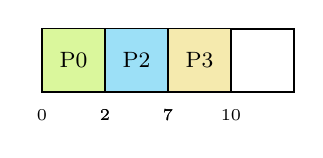
\begin{tikzpicture}%
\draw[thick] (0,0) rectangle (3.200000, 0.800000);%
\node[draw, minimum width=0.800000cm, minimum height=0.800000cm, text centered, fill=P0, font=\fontsize{8}{9}\selectfont] at (0.400000, 0.400000) {P0};%
\node[font=\fontsize{6}{8}\selectfont] at (0.000000, -0.3) {0};%
\node[font=\fontsize{6}{8}\selectfont] at (0.800000, -0.3) {2};%
\node[draw, minimum width=0.800000cm, minimum height=0.800000cm, text centered, fill=P2, font=\fontsize{8}{9}\selectfont] at (1.200000, 0.400000) {P2};%
\node[font=\fontsize{6}{8}\selectfont] at (0.800000, -0.3) {2};%
\node[font=\fontsize{6}{8}\selectfont] at (1.600000, -0.3) {7};%
\node[draw, minimum width=0.800000cm, minimum height=0.800000cm, text centered, fill=P3, font=\fontsize{8}{9}\selectfont] at (2.000000, 0.400000) {P3};%
\node[font=\fontsize{6}{8}\selectfont] at (1.600000, -0.3) {7};%
\node[font=\fontsize{6}{8}\selectfont] at (2.400000, -0.3) {10};%
\end{tikzpicture}%
\end{figure}

%
\subsection{Time 10: Process P1}%
\label{subsec:Time10ProcessP1}%


\begin{figure}[h!]%
\centering%
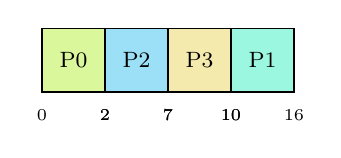
\begin{tikzpicture}%
\draw[thick] (0,0) rectangle (3.200000, 0.800000);%
\node[draw, minimum width=0.800000cm, minimum height=0.800000cm, text centered, fill=P0, font=\fontsize{8}{9}\selectfont] at (0.400000, 0.400000) {P0};%
\node[font=\fontsize{6}{8}\selectfont] at (0.000000, -0.3) {0};%
\node[font=\fontsize{6}{8}\selectfont] at (0.800000, -0.3) {2};%
\node[draw, minimum width=0.800000cm, minimum height=0.800000cm, text centered, fill=P2, font=\fontsize{8}{9}\selectfont] at (1.200000, 0.400000) {P2};%
\node[font=\fontsize{6}{8}\selectfont] at (0.800000, -0.3) {2};%
\node[font=\fontsize{6}{8}\selectfont] at (1.600000, -0.3) {7};%
\node[draw, minimum width=0.800000cm, minimum height=0.800000cm, text centered, fill=P3, font=\fontsize{8}{9}\selectfont] at (2.000000, 0.400000) {P3};%
\node[font=\fontsize{6}{8}\selectfont] at (1.600000, -0.3) {7};%
\node[font=\fontsize{6}{8}\selectfont] at (2.400000, -0.3) {10};%
\node[draw, minimum width=0.800000cm, minimum height=0.800000cm, text centered, fill=P1, font=\fontsize{8}{9}\selectfont] at (2.800000, 0.400000) {P1};%
\node[font=\fontsize{6}{8}\selectfont] at (2.400000, -0.3) {10};%
\node[font=\fontsize{6}{8}\selectfont] at (3.200000, -0.3) {16};%
\end{tikzpicture}%
\end{figure}

%
\subsection{Final Process Table}%
\label{subsec:FinalProcessTable}%
\begin{tabular}{|c|c|c|c|}%
\hline%
\textbf{Process}&\textbf{Arrival Time}&\textbf{Burst Time}&\textbf{Service Time}\\%
\hline%
P0&0&2&0\\%
\hline%
P1&1&6&10\\%
\hline%
P2&2&5&2\\%
\hline%
P3&3&3&7\\%
\hline%
\end{tabular}

%
\subsection{Execution Order}%
\label{subsec:ExecutionOrder}%


\begin{figure}[h!]%
\centering%
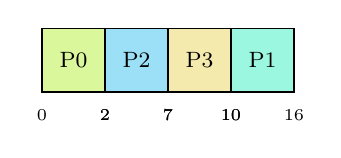
\begin{tikzpicture}%
\draw[thick] (0,0) rectangle (3.200000, 0.800000);%
\node[draw, minimum width=0.800000cm, minimum height=0.800000cm, text centered, font=\fontsize{8}{9}\selectfont, fill=P0] at (0.400000, 0.400000) {P0};%
\node[font=\fontsize{6}{8}\selectfont] at (0.000000, -0.3) {0};%
\node[font=\fontsize{6}{8}\selectfont] at (0.800000, -0.3) {2};%
\node[draw, minimum width=0.800000cm, minimum height=0.800000cm, text centered, font=\fontsize{8}{9}\selectfont, fill=P2] at (1.200000, 0.400000) {P2};%
\node[font=\fontsize{6}{8}\selectfont] at (0.800000, -0.3) {2};%
\node[font=\fontsize{6}{8}\selectfont] at (1.600000, -0.3) {7};%
\node[draw, minimum width=0.800000cm, minimum height=0.800000cm, text centered, font=\fontsize{8}{9}\selectfont, fill=P3] at (2.000000, 0.400000) {P3};%
\node[font=\fontsize{6}{8}\selectfont] at (1.600000, -0.3) {7};%
\node[font=\fontsize{6}{8}\selectfont] at (2.400000, -0.3) {10};%
\node[draw, minimum width=0.800000cm, minimum height=0.800000cm, text centered, font=\fontsize{8}{9}\selectfont, fill=P1] at (2.800000, 0.400000) {P1};%
\node[font=\fontsize{6}{8}\selectfont] at (2.400000, -0.3) {10};%
\node[font=\fontsize{6}{8}\selectfont] at (3.200000, -0.3) {16};%
\end{tikzpicture}%
\end{figure}

%
\end{document}